\documentclass[10pt,aspectratio=169]{beamer}
\usepackage{xcolor}
\definecolor{darkblue}{RGB}{0,37,70}
\definecolor{darkred}{RGB}{70,0,38}
\definecolor{darkorange}{RGB}{231,129,0}
\definecolor{darkbrown}{RGB}{108,60,0}
\definecolor{darkgreen}{RGB}{5,130,0}

\usetheme[numbering=fraction,progressbar=head,background=light,block=fill]{metropolis}

\usepackage{etoolbox}

\setbeamercolor{block title}{use=structure,fg=structure.fg,bg=structure.fg!20!bg}
\setbeamercolor{block body}{parent=normal text,use=block title,bg=block title.bg!50!bg}

\setbeamercolor{block title example}{use=example text,fg=example text.fg,bg=example text.fg!20!bg}
\setbeamercolor{block body example}{parent=normal text,use=block title example,bg=block title example.bg!50!bg}

\BeforeBeginEnvironment{theorem}{
    \setbeamercolor{block title}{fg=normal text.fg,bg=structure.fg!10!bg}
    \setbeamercolor{block body}{fg=normal text.fg, bg=white!97!black}
}
\AfterEndEnvironment{theorem}{
 \setbeamercolor{block title}{use=structure,fg=structure.fg,bg=structure.fg!20!bg}
 \setbeamercolor{block body}{parent=normal text,use=block title,bg=block title.bg!50!bg, fg=normal text.fg}
}

\setbeamercolor{normal text}{%
	fg=darkblue,
	bg=white
}

\setbeamercolor{title page text}{
	fg=white,
	bg=transparent}

\usepackage{pgfpages}

\usepackage[numbers,square,sort&compress]{natbib}
\usepackage[american]{babel}
\setbeamertemplate{bibliography item}{\insertbiblabel}

% \usepackage{booktabs}
\usepackage{algorithmic}

% Definitions
\newcommand{\myparallel}{\textcolor{darkbrown}{parallel}}
\newcommand{\mysequential}{\textcolor{darkgreen}{sequential}}

\newcommand{\obj}{\mathcal{O}}
\newcommand{\kl}{D_{KL}}
\newcommand{\proxy}{\mathcal{P}}
\newcommand{\R}{\mathbb{R}}
\newcommand{\orth}{\mathcal{O}}
\newcommand{\I}{\mathbb{1}}
% \newcommand{\C}{\mathbb{C}}
\newcommand{\E}{\mathbb{E}}
\newcommand{\lrelu}{\text{LeakyReLU}}
\newcommand{\bias}{\text{Bias}}
\newcommand{\cnn}{\text{CNN}}
\newcommand{\eps}{\varepsilon}
\newcommand{\conv}{\text{conv}_{3d}}
\newcommand{\convtwo}{\text{conv}_{2d}}
\newcommand{\dft}{\text{DFT}_{3d}} % default is 3, add 2 also. 
\newcommand{\idft}{\text{DFT}^{-1}_{3d}}
\newcommand{\channels}{\text{\# channels}}
\DeclareMathOperator*{\argmax}{\arg{}\,\max}
\DeclareMathOperator*{\argmin}{\arg{}\,\min}
% end definitions

% \setbeameroption{show notes on second screen}
% \makeatletter
% \def\beamer@framenotesbegin{% at beginning of slide
% \usebeamercolor[fg]{normal text}
% \gdef\beamer@noteitems{}%
% \gdef\beamer@notes{}%
% }
% \makeatother


\title{Fast, Effective and Interpretable Deep Learning}

\date{\today}
\author{Frederik Hvilshøj}
% \institute{Aarhus University, Department of Computer Science}
\titlegraphic{\vspace{4.3cm}\hspace{9.8cm}
\includegraphics[width=0.5\textwidth]{logo.png}}

\begin{document}

\maketitle

% TOC
\begin{frame}{Table of contents}
  \setbeamertemplate{section in toc}[sections numbered]
  \tableofcontents[hideallsubsections]
\end{frame}

\section{Introuction}
\begin{frame}{Introduction}
	\begin{itemize}
		\item Deep Learning is \alert{leading paradigm} in Machine Learning
		\item Much effort put into network \alert{design} and \alert{efficiency}
		\item Models may be \alert{biased} due to model constraints
		\item Limited insights -- knowledge is based on \alert{intuition}
		\item \alert{Explanations} are important for sensitive tasks
	\end{itemize}
\end{frame}


\begin{frame}{This Project}
	\begin{columns}
		\begin{column}{0.45\textwidth}
			\begin{itemize}
				\item Explanations of general neural network is challenging
				\item Invertible functions give a higher level of insights
			\end{itemize}
		\end{column}
		\begin{column}{0.45\textwidth}
			\centering
			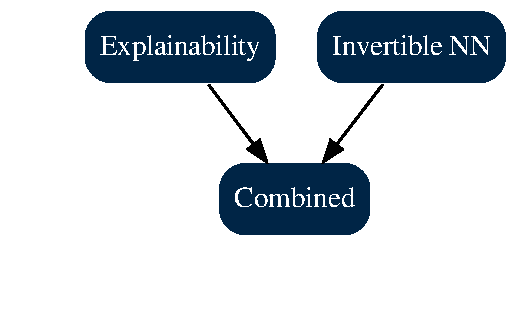
\includegraphics[width=\textwidth]{project}
		\end{column}
	\end{columns}
\end{frame}


\section{Normalizing Flows}
\begin{frame}{Normalizing Flows}
 	\alert{Goal:} Learn a representation of a density $p(x)$ 

	\alert{Model:} Maximize log-likelihood of the data with respect to the parameters of an invertible Neural Network $f$.

	$$
		\log( p_\theta(x) ) = \log( p_z(f(x)) ) + \log( | det \frac{\partial f(x)}{\partial x}| )
	$$

	\alert{Constraints:} invertible $f$ and tractable Jacobian.


	$$
		log\left( | \det  \frac{\partial f_k(f_{k-1}(\dots f_1(x)))}{\partial x} | \right) = \sum_{i=1}^k \log \left( | \det \frac{\partial f_i(z_{i-1})}{\partial z_{i-1}} | \right)
	$$

	$$
		z_0 = x, \quad z_i = f_{i}(z_{i-1})
	$$
\end{frame}

\begin{frame}{Normalizing Flow Layers}
	\begin{description}
		\item[Coupling layer] $c(x) = (x_1, x_2 + m(x_1))$, for $x = (x_1, x_2)$~\cite{nice}
		\item[Channel permutation] Fixed channel permutations of 3D data~\cite{realnvp}
		\item[1x1 convolutions] Learnable channel interactions~\cite{glow}
		\item[Periodic convolutions] Circular convolutions over each channel~\cite{emerging}
	\end{description}
\end{frame}

\begin{frame}[standout]
	What if Neural Networks had SVDs?
\end{frame}

\begin{frame}{The Singular Value Decomposition}
	\begin{definition}
		The Singular Value Decomposition of $W \in \R^{m\times n}$ is a factorization
		$W = U \Sigma V^T$, where  $U$ is an \alert{orthogonal} $m \times m$ matrix,
		$\Sigma$ is an $m \times n$ rectangular diagonal matrix, and $V$ is an $n \times
		n$ \alert{orthogonal} matrix.
	\end{definition}
\end{frame}

\begin{frame}{Properties of the SVD}
	For out purposes, assume that $W$ is a square, i.e., $W \in \R^{d\times d}$.
	Then:
	\begin{align*}
		U^{-1} &= U^T\text{ and }V^{-1} = V^T  \quad \quad & O(d^2)\\
		W^{-1} &= (U \Sigma V^T)^{-1} = V \Sigma^{-1} U^T  & O(d^2)\\
		det(W) &= \prod_{i=1}^{d} \Sigma_{i,i}   & O(d)
	\end{align*}
	Other fast computations are largest singular value, condition number, matrix exponential, and Cayley Map.
\end{frame}

\begin{frame}{Use in Neural Networks}
	% Titles
	\begin{columns}
		\begin{column}{0.47\textwidth}
			\alert{Neural Networks}
		\end{column}
		\begin{column}{0.47\textwidth}
			\alert{Gradients}
		\end{column}
	\end{columns}
	\vspace{1em}

	\begin{columns}
		\begin{column}{0.47\textwidth}
			Recall a simple fully-connected layer:
			\begin{equation*}
 				h_{\ell} = \sigma (Wh_{\ell-1}) = \sigma \left( U\Sigma V^T h_{\ell-1}\right)
			\end{equation*}

			\begin{itemize}
				\item Normalizing flows
				\item Recurrent Neural Networks
				\item W-GAN
			\end{itemize}
		\end{column}

		\begin{column}{0.47\textwidth}
			% What happens when we use gradient descent?
			\begin{align*}	
				W^{t+1} &= W^{t} - \eta \frac{\partial L}{\partial W}\\
				\Sigma^{t+1} &= \Sigma^{t} - \eta \frac{\partial L}{\partial \Sigma}\\
				U^{t+1} &= U^{t} - \eta \frac{\partial L}{\partial U}\\
			\end{align*}
		\end{column}
	\end{columns}
\end{frame}

\begin{frame}{The Householder Matrix}
	\begin{definition}
 		For a vector $v \in \R^{d}$, the corresponding Householder matrix
 		is defined as
 		\begin{equation}\label{eq:hh}
 			H = I - 2\frac{v v^T}{||v||^2_2}
 		\end{equation}
	\end{definition}

	\begin{itemize}
		\item Note LHS of Eqn. (\ref{eq:hh}) takes $O(d^2)$ but RHS takes $O(d)$.
		\item $H$ stays orthogonal under gradient descent on $v$!
	\end{itemize}

	\begin{lemma}
		The product of two orthogonal matrices is orthogonal. 
	\end{lemma}
\end{frame}

\begin{frame}{Main Idea}
	Parametrize $U$ and $V$ as a product of Householder matrices \cite{orthhh}.
	
	$$
		U = H_1 \cdot H_2 \cdots H_{d}
	$$

	When evaluating a NN, we need to compute

	$$
		UX = H_1 ( H_2 ( \cdots (H_{d} X)))
	$$

	with $X \in \R^{d \times m}$, where $m$ is the batch size.

	If we represent $H_i$s as matrices, this takes $O(d^3m)$ time (denoted \myparallel~\cite{orthhh}).
	We can easily improve by representnig $H_i$ by its vectors
	$v_i$ instead, $O(d^2m)$ (denoted \mysequential~\cite{orthhh}).
	%$v_i$ instead, $O(d^2m)$ (denoted \emph{sequential}).
\end{frame}

\begin{frame}{Issues}
	
	\textbf{Issues:}
	\begin{itemize}
		\item The \myparallel~algorithm is slow in theory.
		\item The \mysequential~algorithm is not suited for GPUs.
	\end{itemize}

	\textbf{We propose:}
	\begin{itemize}
		\item Algorithm which is suited for GPUs and fast in theory.
	\end{itemize}

\end{frame}

\begin{frame}{Our Algorithm}

	\begin{lemma}
		\cite{wydec} For any $m$ Householder matrices $H_1,...,H_m$ there exists $W,Y\in \R^{d\times m}$ st. 
		$$I-2WY^T = H_1 \cdots H_m. $$
		Both $W$ and $Y$ can be computed by $m$ sequential Householder multiplications in $O(dm^2)$ time. 
	\end{lemma}

	\begin{center}
		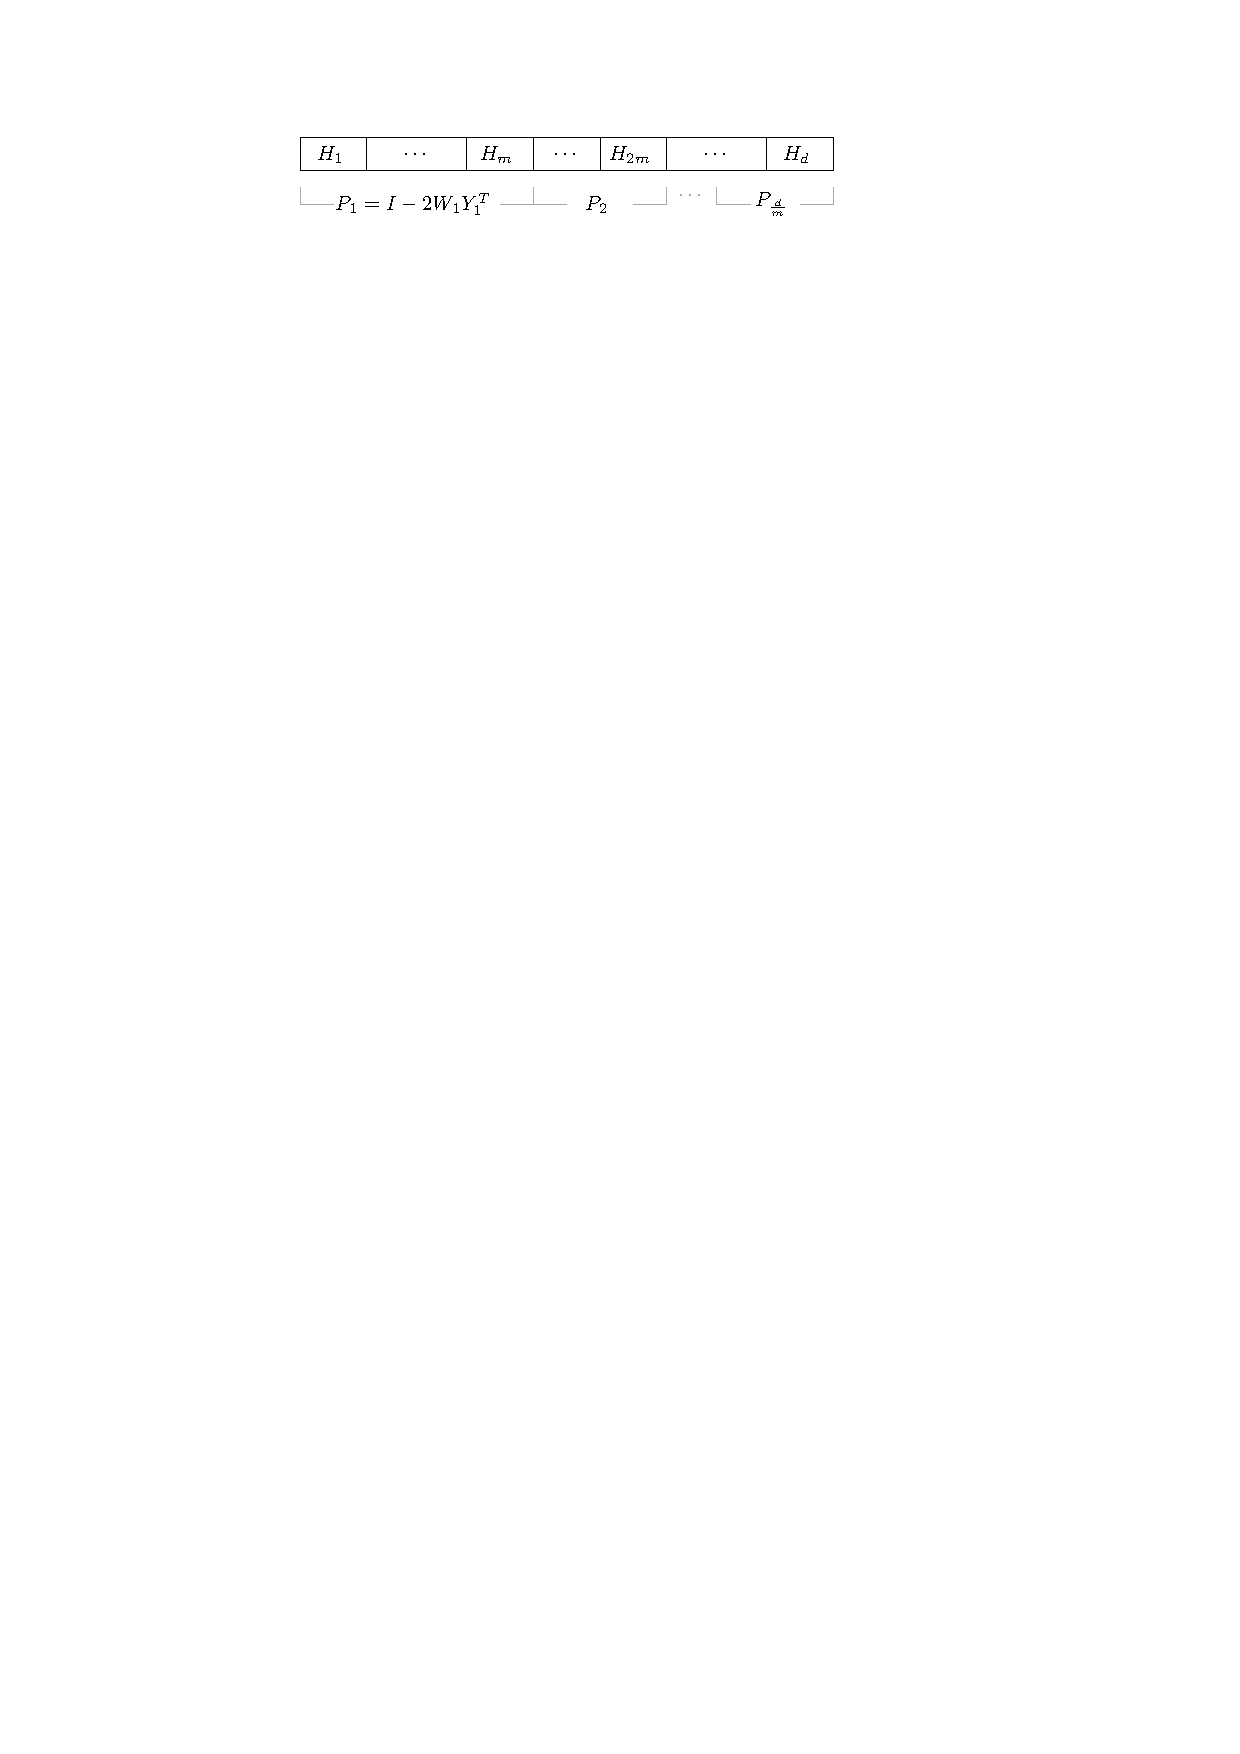
\includegraphics[width=0.7\textwidth, page=1]{graphics}
	\end{center}

\end{frame}

\begin{frame}{Complexity}

		\textbf{Time:} 
		$$P_1 \cdot P_2 \cdots P_{\frac{d}{m}} X \qquad O(d^3m) \Rightarrow O(d^2m) $$
		\textbf{\# sequential opetations:} 
		$$O(\text{compute }I-2WY^T + \text{multiply }P_i\text{s}) = O(d/m + m)$$

\end{frame}

\begin{frame}{Experiments}
	\begin{columns}
		\begin{column}{0.49\textwidth}
			\vspace{1em}
			\centering
			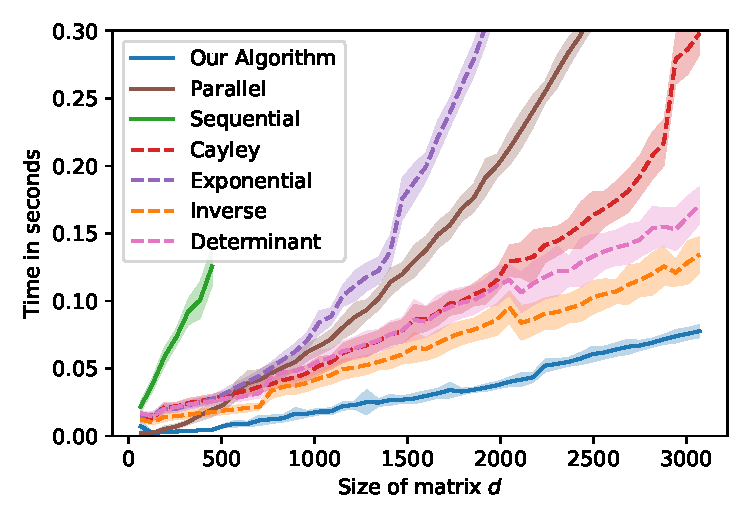
\includegraphics[width=\textwidth]{matrix_operations}
		\end{column}
		\begin{column}{0.49\textwidth}
			\vspace{1em}
			\centering
			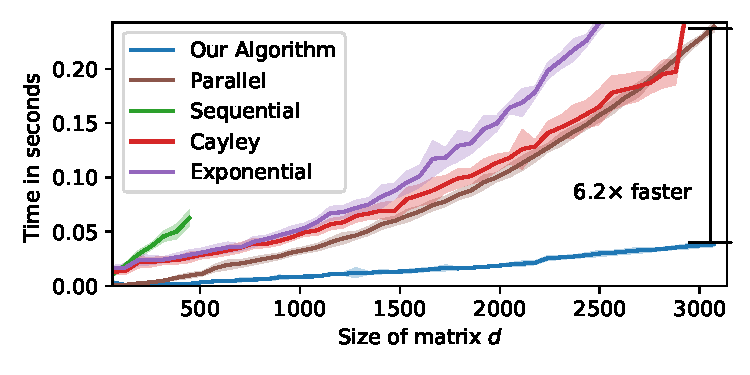
\includegraphics[width=\textwidth]{running_time}
			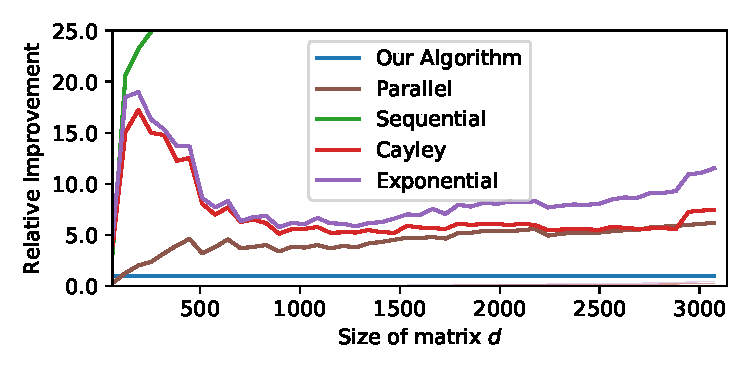
\includegraphics[width=\textwidth]{relative}
		\end{column}
	\end{columns}
\end{frame}



\begin{frame}[standout]
	Circular 3D Convolutions
\end{frame}

\begin{frame}{3D Circular Convolutions}
    \begin{center}
    	\includegraphics[width=0.75\textwidth,page=3]{convolutions_wpurple.pdf}	
    \end{center}

    \alert{Algorithm:} Forward $O(hwc \log hwc)$, Determinant $O(hwc)$
    \begin{algorithmic}[1]
  	  %\SetAlgoLined
		\REQUIRE{Image/activations $X\in\R^{h\times w \times c}$ and kernel $K\in\R^{h\times w\times c}$}.
		\STATE $X$ = DFT$_{3D}$($X$) 
		\STATE $K$ = DFT$_{3D}$($K$)
		\STATE $X$ = $X \odot  K$  
		\STATE $X$ = DFT$_{3D}^{-1}$($X$) 
	\end{algorithmic}
\end{frame}

\begin{frame}{Comparison with Periodic Convolutions}
	For $X, K \in \R^{h \times w \times c}$ and $W \in \R^{c \times c \times h \times w}$

	\alert{Circular 3D connvolutions}
	$$
		Z = F_{3D}^{-1}(F_{3D}(X) \odot F_{3D}(K))
	$$

	\alert{Periodic convolutions}
	$$
		z_{i} = F_{2D}^{-1}( \sum_{j=1}^c F_{2D}(W_{i, j}) \odot F_{2D}(X_{:,:,j})),
	$$

	\begin{center}
		\begin{tabular}{c|c c c c }
        	Type & Params & Forward & Inverse\\
    	\hline
        	Periodic & $h\cdot w \cdot c^2$ & $O(hwc^2)$ & $O(hwc^3)$ \\
        	3D-circular$^\dagger$ & $h \cdot w \cdot c^2$ & $O(hwc^2 \log (hwc))$ & $O(hwc^2 \log (hwc))$ \\
    	\end{tabular}
    \end{center}
	%\begin{tabular}{llll}
	%	\toprule
	%		Type &  Evaluation & Inversion & Log-determinant \\
	%	\midrule
	%	%1x1     &  $F_{1d}^{-1}\left[F_{1d}(x_{ij})\odot F_{1d}(k)\right]$ & $F_{1d}^{-1}(F_{1d}(x_{ij})\odot 1/F_{1d}(k))$  & $hw\sum_i \log (|F_{1d}(k)_i|$ \\
	%		3D      & $F^{-1}(F(X) \odot F(K))$ &  $F^{-1}(F(X) \odot 1/F(K))$  & $\sum_{ijk} \log(|F(K)_{ijk}|)$ \\
	%\end{tabular}
\end{frame}


\begin{frame}[standout]
	Improving Variational Auto-Encoders
\end{frame}

\begin{frame}{Improving Variational Auto-Encoders}
	Variational lower-bound:
	$$
		\log p(x) \geq \E_{z \sim q(z | x)}\left[ \log p(x | z) \right] + D_{KL}(q(z|x) || p(z))
	$$

	where $q(z|x) = \mathcal{N}(\mu(x), diag(\sigma(x)))$.

	With formalizing flow $f$, the equation becomes

	$$
	\log p(x) \geq  \E_{z\sim p(z|x)}\left[ \log p(x|f(z)) + \log |Det\frac{\partial f(z)}{\partial z}|\right] + D_{KL}\left(q(z|x) || p(f(z))\right)
	$$

	\cite{houseVAE} let $f(z) = H_TH_{T-1}\cdots H_1z$ with each $H_i$ being parametrized by the encoder.
	
\end{frame}

\begin{frame}{Improving Variational Auto-Encoders}
	\begin{figure}
		\centering
		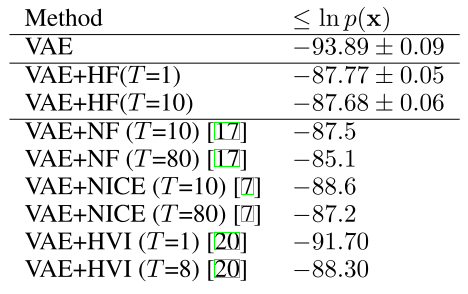
\includegraphics[width=0.4\textwidth]{houseVAE}
		\caption{Comparison of the lower bound of marginal log-likelihood measured in nats of the digits in the MNIST test set. For the first three methods the experiment was repeated 3 times. \alert{Direct copy from \cite{houseVAE}.}}
	\end{figure}
\end{frame}


\section{Explainability}
\begin{frame}{Explanations}
	Here we focus on \alert{explainability}, characterized by
	\vspace{1em}

	\begin{quote}
		An active characteristic of a model, denoting any action or procedure taken by a model with the intent of clarifying or detailing its internal functions~\cite{Arrieta2019}.
	\end{quote}

	We consider \alert{attribution} techniques and \alert{counterfactual} explanations. 

\end{frame}

\begin{frame}{Attribution Techniques}
	\begin{itemize}
		\item Identifies contribution of each input feature wrt. the output
		\item ``Gradient-like'' computations
		\item Based on different propagation rules
	\end{itemize}
	
	\begin{figure}
		\centering
		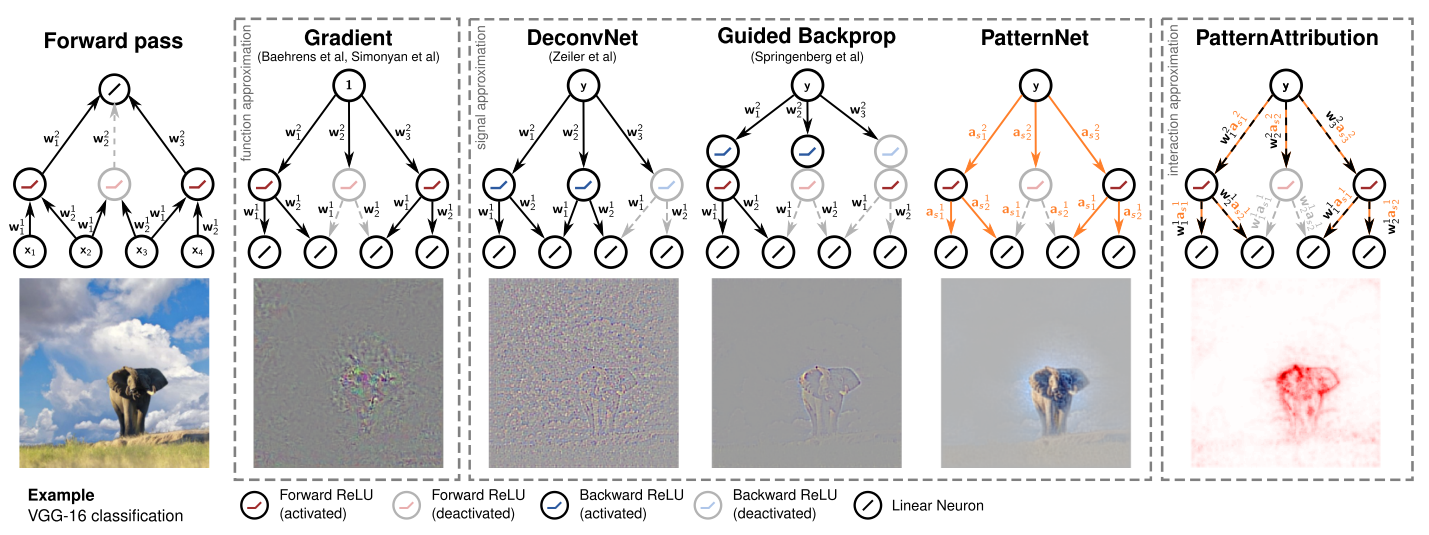
\includegraphics[width=0.8\textwidth]{explanation_techniques}
		\caption{Direct copy from~\cite{patternnet}.}
	\end{figure}
\end{frame}

\begin{frame}{Counterfactual Explanations}

	Counterfactual explanations tries to answer the question 
	\vspace{1em}

	\begin{quote}
		How can I make a \alert{minimal} and \alert{realistic} change to an input of the model such that the predicted outcome changes?
	\end{quote}
	\vspace{1em}

	\begin{columns}
		\begin{column}{0.5\textwidth}
			\alert{Common strategy}
			\begin{enumerate}
				\item Start from the original input
				\item Until prediction change
					\begin{enumerate}
						\item Make small change to the input
						\item Query the classifier to gain information
					\end{enumerate}
			\end{enumerate}
		\end{column}
		\begin{column}{0.5\textwidth}
			\alert{Differences}
			\begin{itemize}
				\item How to do update
				\item Information gained from classifier
			\end{itemize}
		\end{column}
	\end{columns}

\end{frame}

\begin{frame}[standout]
	Improving Explanations with Probabilistic Saliency Estimation
\end{frame}

\begin{frame}{Probabilistic Saliency Estimation}

\end{frame}

\begin{frame}{Area Under Perturbation Score}

\end{frame}

\begin{frame}[standout]
	Attention Mechanisms in Gradient Explanations
\end{frame}

\begin{frame}{Explanations Relies on Gradients}
	% Generalization
	% Guided Back Prop as example
\end{frame} 





\begin{frame}{Issues}
	% Loss for attribution functions?
\end{frame}

\begin{frame}[standout]
	Generating Counterfactual Explanations
\end{frame}


\begin{frame}{Construction}
	$$
	f(x) = \sigma \left ( \beta^T NN(x) \right)
	$$

	$$
	f^\dagger(y) = NN^{-1}\left( f(x) - \frac{f(x)^T \beta}{||\beta||}\right)
	$$
\end{frame}




\appendix
\begin{frame}[t, allowframebreaks]{References}
	\bibliographystyle{plainnat} 
	\begingroup
	\renewcommand{\section}[2]{}%
	\footnotesize
	\bibliography{references}
	\endgroup

	% \bibliography{references}
\end{frame}

\begin{frame}{Attention example}
	\begin{center}
		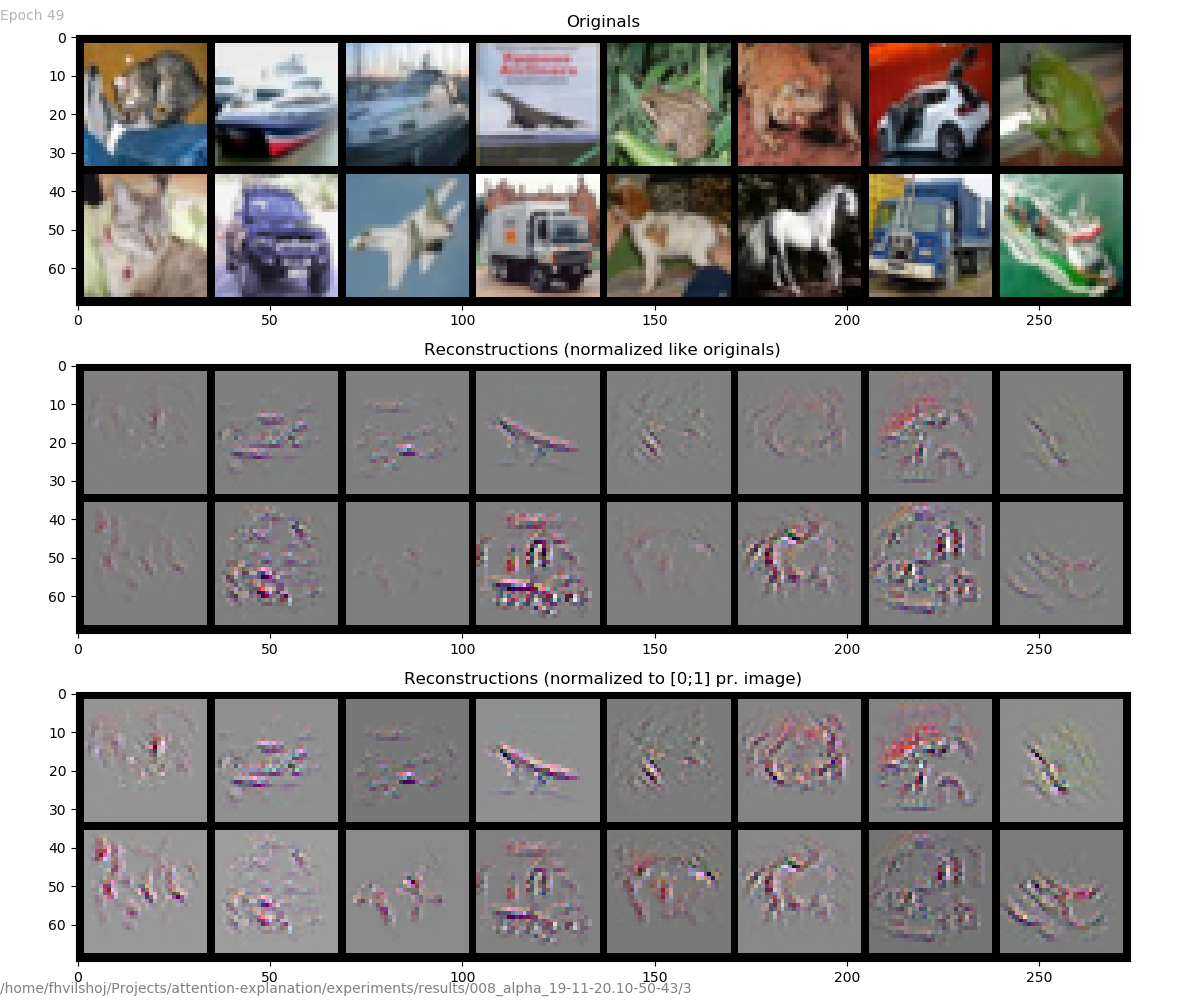
\includegraphics[width=0.6\textwidth]{ex1}
	\end{center}
\end{frame}

\begin{frame}{Attention example}
	\begin{figure}
		\centering
		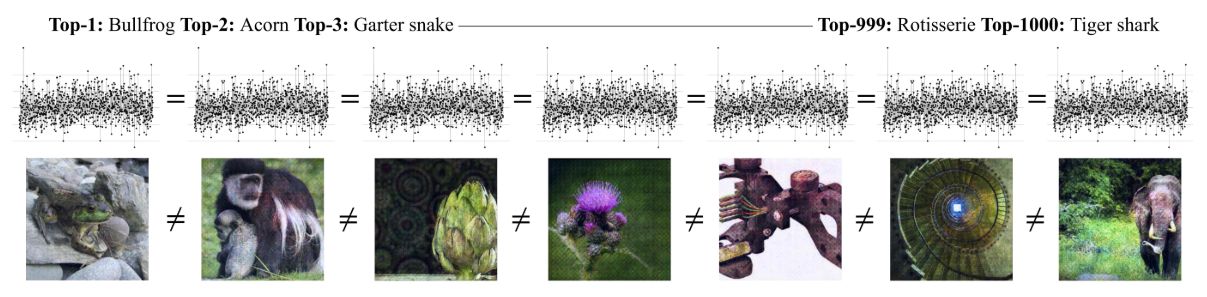
\includegraphics[width=\textwidth]{excessive}
		\caption{Direct copy from~\cite{Jacobsen2019}.}
	\end{figure}
\end{frame}

\end{document}

